\section{Versuchsauswertung}
%
\subsection{Einleitung und Zielsetzung}

Die im Labor aufgenommenen Messwerte und die mithilfe des KiCads erstellten Simulationswerte werden in diesem Abschnitt für verschiedene Arten des Filters dargestellt. Durch den Vergleich der Messwerten sowie der Simulationsergebnissen mit der Theorie wird die Realisierung verschiedener Filterarten genauer untersucht.

%

\subsection{Der Integrator}

In der Abbildung \ref{fig:invertierender Integrator_Simulation} wurde das Bodediagramm der simulierten Integrator-Schaltung(\ref{fig:invertierender Integrator}) zusammen mit den aufgenommenen Messwerten dargestellt.

\begin{figure}[H]
  \centering
  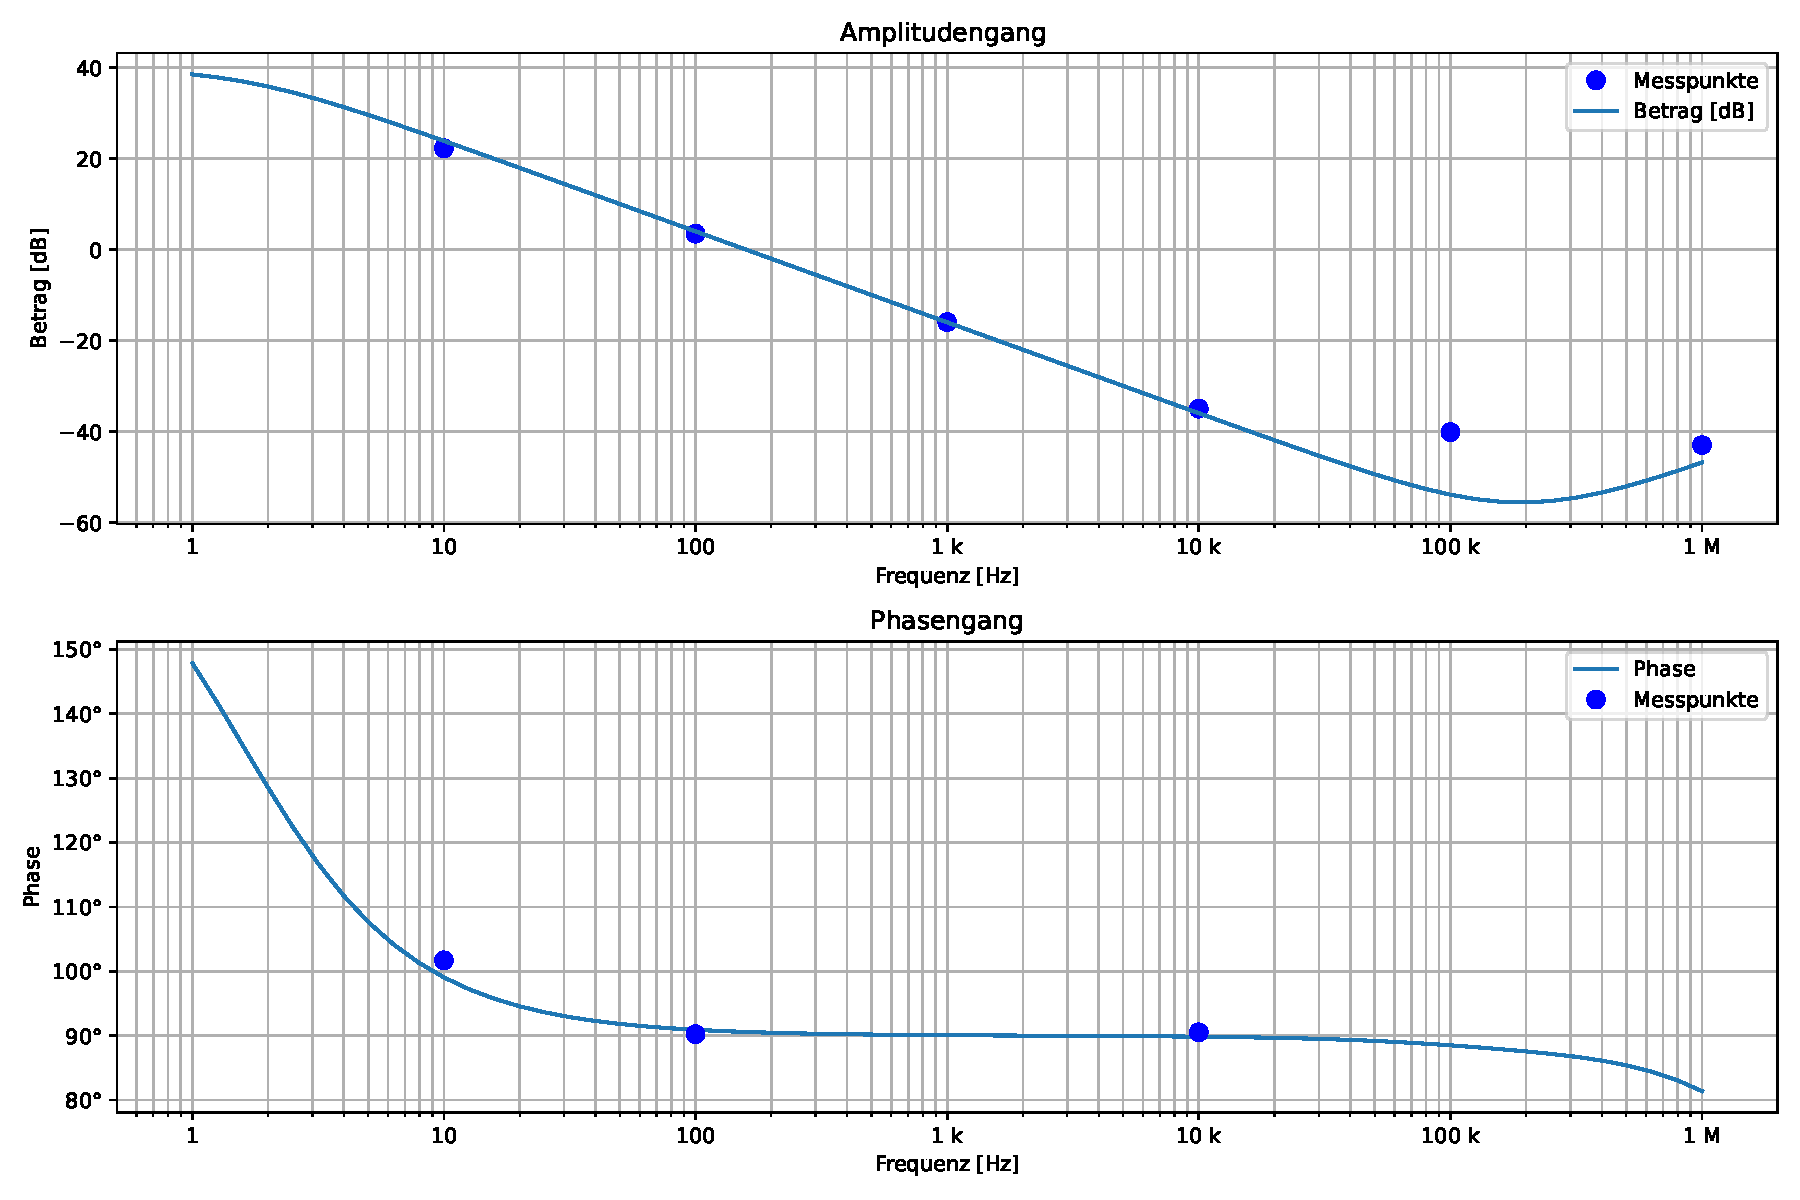
\includegraphics[width=0.8\linewidth]{Elektronik-Laborprotokoll_Filter/Plots/invertierender_Integrator_mit_Messwerten.pdf}
  \caption{invertierender Integrator Simulation mit gemessenen Werten}
  \label{fig:invertierender Integrator_Simulation}
\end{figure}
%
Bei der Integrator-Schaltung ist die Amplitudenverstärkung für tiefere Frequenzen größer. Wenn sich die Frequenz des Eingangssignals an die \SI{0}{\hertz} nähert, läuft die Verstärkeung des Integrators gegen unendlich. Die Verstärkung des Integrators verringert sich um \SI{20}{\decibel} pro Dekade.

Die Ausgangsspannung eines invertierenden Integrators steht in Beziehung zur Eingangsspannung gemäß der folgenden Formel\cite{Skript}:

\begin{equation}
U_a(t) = -\frac{1}{RC} \int_{0}^{t} U_e(t) \, dt
\end{equation}


Die komplexe Übertragungsfunktion des Integrators hat die folgende Form:

\begin{equation*}
    H_{int}(s)=\frac{-1}{sRC} 
\end{equation*}
\begin{equation}
\label{eq:Übertragung}
   H_{int}(j\omega)=\frac{-1}{j\omega R_1C}
\end{equation}

Die Integratorverstärkung ist im Bodediagramm mit \( \left| H_{int}(j\omega) \right| \) in \si{\decibel} dargestellt. Mit der Formel \ref{eq:Übertragung} kann man die Grenzfrequenz $f_g$ berechnen, wobei die Amplitudenverstärkung gleich 1 ist, bzw. die Amplitude des Ausgangssignal gleich groß wie die Amplitude des Eingangssignals ist.

Die Frequenz $f$ hängt mit der Kreisfrequenz $\omega$ unter folgender Gleichung zusammen:
\begin{equation}
\label{eq:Frequenz}
    f=\frac{\omega}{2\pi}
\end{equation}
Die Grenzfrequenz $f_g$ lässt sich berechnen, indem die Gleichung \ref{eq:Frequenz} in die Gleichung \ref{eq:Übertragung} für \( \left| H_{int}(j\omega) \right| \)$=1$ eingesetzt wird:
\begin{equation*}
 f_g=\frac{1}{2\pi R_1C}=\frac{1}{2\pi \cdot \SI{10}{\kilo\ohm} \cdot \SI{100}{\nano\farad}}\approx \SI{159}{\hertz}  
\end{equation*}

Wenn man den Amplitudengang des Integrators untersucht, kann man bestätigen, dass sich die Grenzfrequenz $f_g$ genau wie nach den theoretischen Überlegungen bei  \SI{159}{\hertz} befindet. Die durch die im Labor aufgenommenen Messwerte ermittelten Messpunkte stimmen sehr gut mit der Simulationskurve überein, bis auf kleine Abweichungen bei höheren Frequenzen. Diese Abweichung liegt wahrscheinlich daran, dass sehr kleine Ausgangsspannung bei höheren Frequenzen die genauere Bestimmung seiner Größe schwieriger macht.

 Wenn sich die Frequenz des Eingangssignals an die \SI{0}{\hertz} nähert, läuft der Phasenunterschied des Integrators gegen \SI{180}{\degree}. Die Verstärkung des Integrators verringert sich mit steigender Frequenz bis auf \SI{90}{\degree}. Ein Phasenunterschied zwischen Eingang und Ausgangsignals  von \SI{90}{\degree} wird genau bei der Grenzfrequenz erreicht. Die durch die im Labor aufgenommenen Messwerte ermittelten Messpunkte stimmen sehr gut mit der Simulationskurve überein, jedoch konnte der Phasenunterschied für sehr hohe Frequenzen ab \SI{100}{\kilo\hertz} am Oszilloskop bzw. mithilfe der aufgenommenen Messdaten nicht exakt bestimmt werden.

 


 



%
\subsection{Aktive Filter erster Ordnung}


In der Abbildung \ref{fig:Tiefpassfilter_Bodediagramm} wurde das Bodediagramm des Tiefpassfilters (\ref{fig:circuit_Tiefpass}) für die Simulation-, und Messwerte dargestellt.

\begin{figure}[H]
  \centering  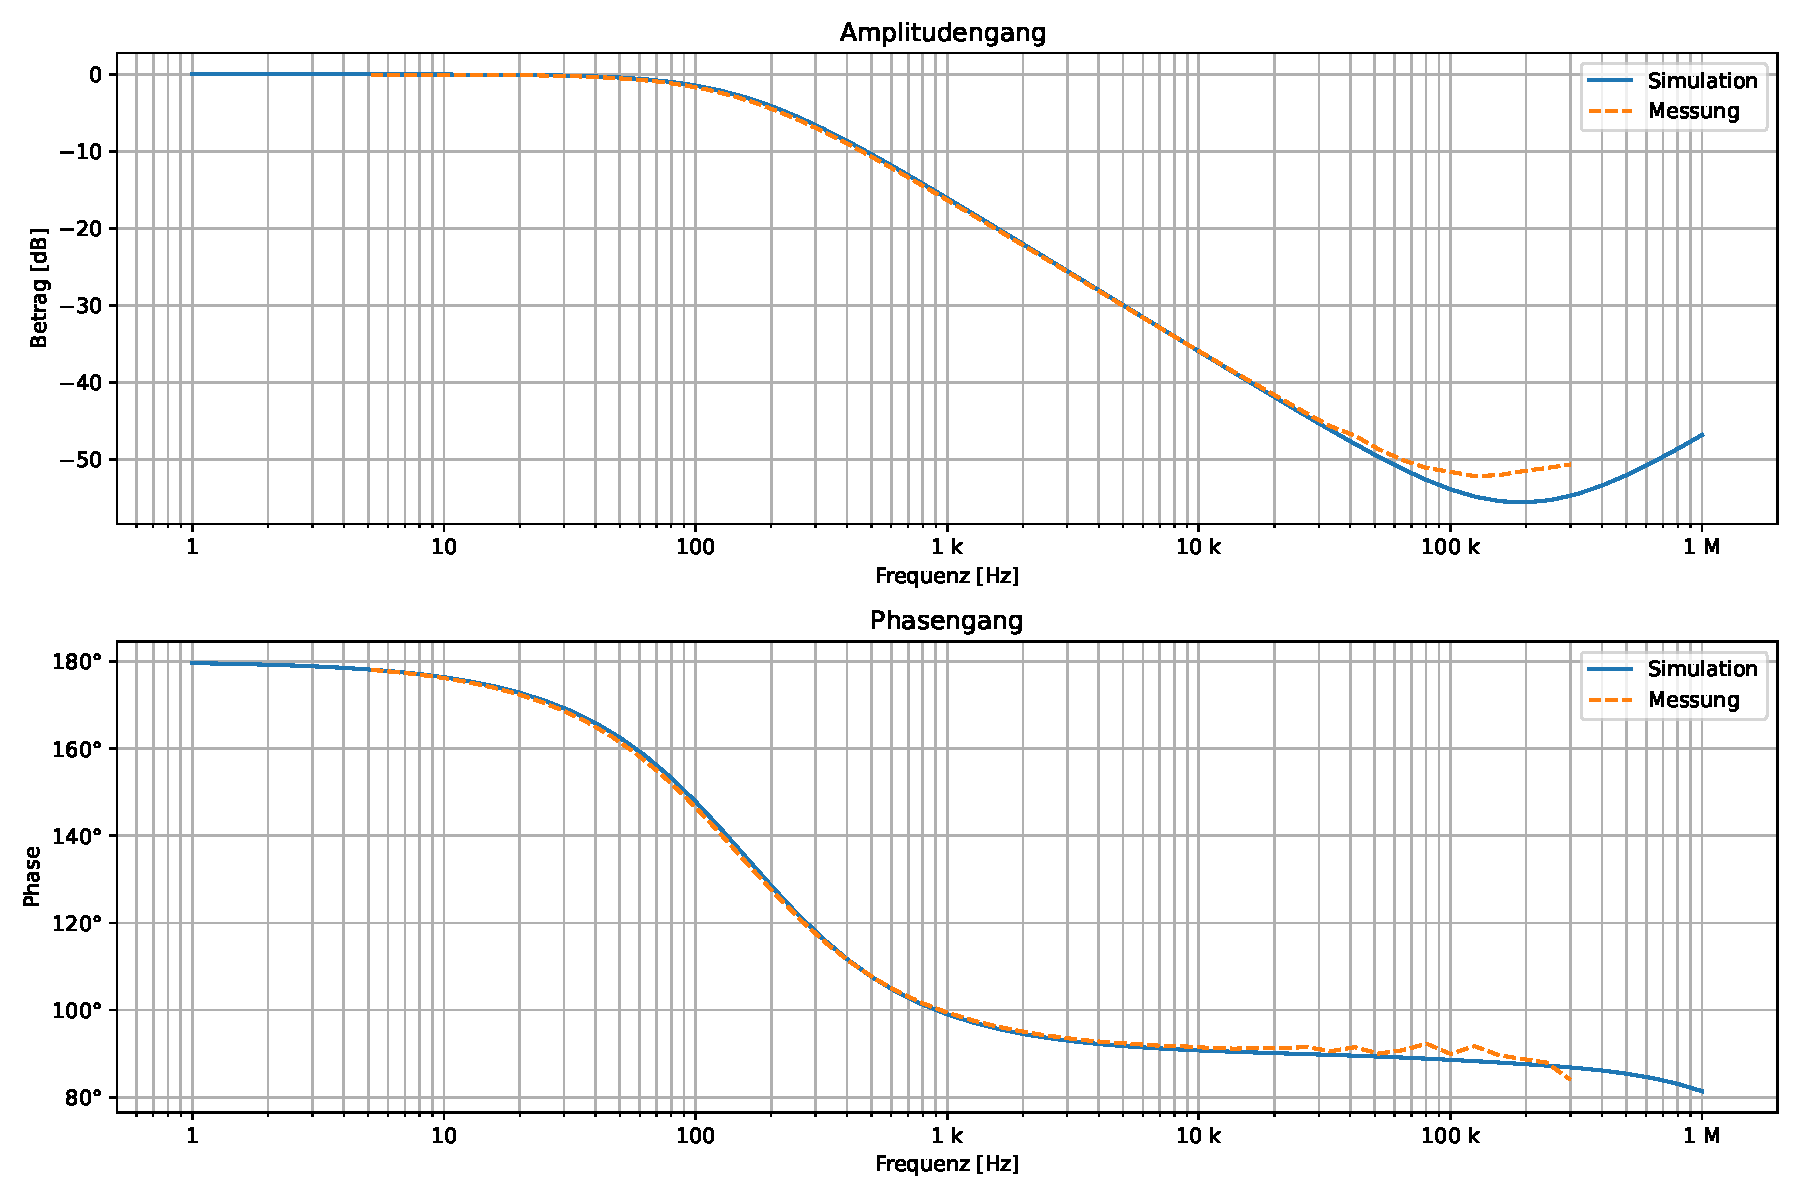
\includegraphics[width=0.8\linewidth]{Elektronik-Laborprotokoll_Filter/Plots/Tiefpass_Bodediagramm_Simulation_mit_Messung.pdf}
  \caption{Tiefpassfilter Bodediagramm}
  \label{fig:Tiefpassfilter_Bodediagramm}
\end{figure}

Mithilfe eines Tiefpassfilters wird es ermöglicht, höhere Frequenzanteile der Signale zu dämpfen, wenn die tiefere Frequenzanteile unverändert durch das Filter durchlaufen können.\\
%
Aus einem Integrator baut man ein aktives Tiefpassfilter erster Ordnung, indem man den Widerstand $R_2$, der sich parallel zum Kondensator befindet, richtig dimensioniert.\\
%
Die komplexe Übertragungsfunktion des Tiefpassfilters erster Ordnung hat die folgende Form:

\begin{equation*}
    H_{int}(s)=-\frac{R_2}{R_1}\cdot\frac{1}{1+sR_2C} 
\end{equation*}
\begin{equation}
\label{eq:Übertragung_Filter}
   H_{int}(j\omega)=-\frac{R_2}{R_1}\cdot\frac{1}{1+j\omega R_2C} 
\end{equation}

Das Tiefpassfilter ist im Bodediagramm mit \( \left| H_{int}(j\omega) \right| \) in \si{\decibel} dargestellt. Mit der Formel \ref{eq:Übertragung} kann man die Grenzfrequenz $f_g$ berechnen. Die Signale mit höherer Frequenzen als  Grenzfrequenz $f_g$ werden stark gedämpft.

Die Grenzfrequenz $f_g$ lässt sich mit folgender Formel berechnen:

\begin{equation*}
 f_g=\frac{1}{R_2 C 2\pi} 
\end{equation*}

und mit der verwendeten Dimensionierung gilt:

\begin{equation*}
 f_g=\frac{1}{\SI{10}{\kilo\ohm}\cdot\SI{100}{\nano\farad}}\approx \SI{159}{\hertz}
\end{equation*}

Die Grenzfrequenz des Tiefpassfilters kann man mithilfe der Dimensionierung der Bauteile $R_2$ und $C$ einstellen.An dem dargestellten Bodediagramm erkennt man, dass die als Signale mit einer Frequenz von kleiner als $f_g= \SI{159}{\hertz}$durch das Filter  unverändert durchgehen darf. Alle anderen höhere Frequenzanteile werden durch das Tiefpassfilter gedämpft. Je höher die Frequenz ist, desto stärker wird das Eingangssignal gedämpft. 

Der Phasenunterschied beträgt bei einer Frequenz, die gegen \SI{0}{\hertz} läuft, \SI{180}{\degree}. Der Phasenunterschied verringert sich bei höheren Frequenzen und er beträgt \SI{135}{\degree} bei der Grenzfrequenz $f_g$. Für höhere Frequenzen verringert sich die Phase weiter und näher sie sich an einen Wert von \SI{90}{\degree}.

Das Bodediagramm, welches mithilfe der im Labor gemessenen Werte erstellt wurde, stimmt mit dem Bodediagramm,  welches mithilfe dersimulierten Werte erstellt wurde, sehr gut überein. Die kleine Abweichung liegt an unverzichtbaren Messungenauigkeiten.


%
\subsection{PI Filter}
In der Abbildung \ref{fig:PI_Filter_Bodediagramm} wurde das Bodediagramm des PI Filters (\ref{fig:PI_Filter_circuit}) für die Simulation-, und Messwerte dargestellt.

\begin{figure}[H]
  \centering  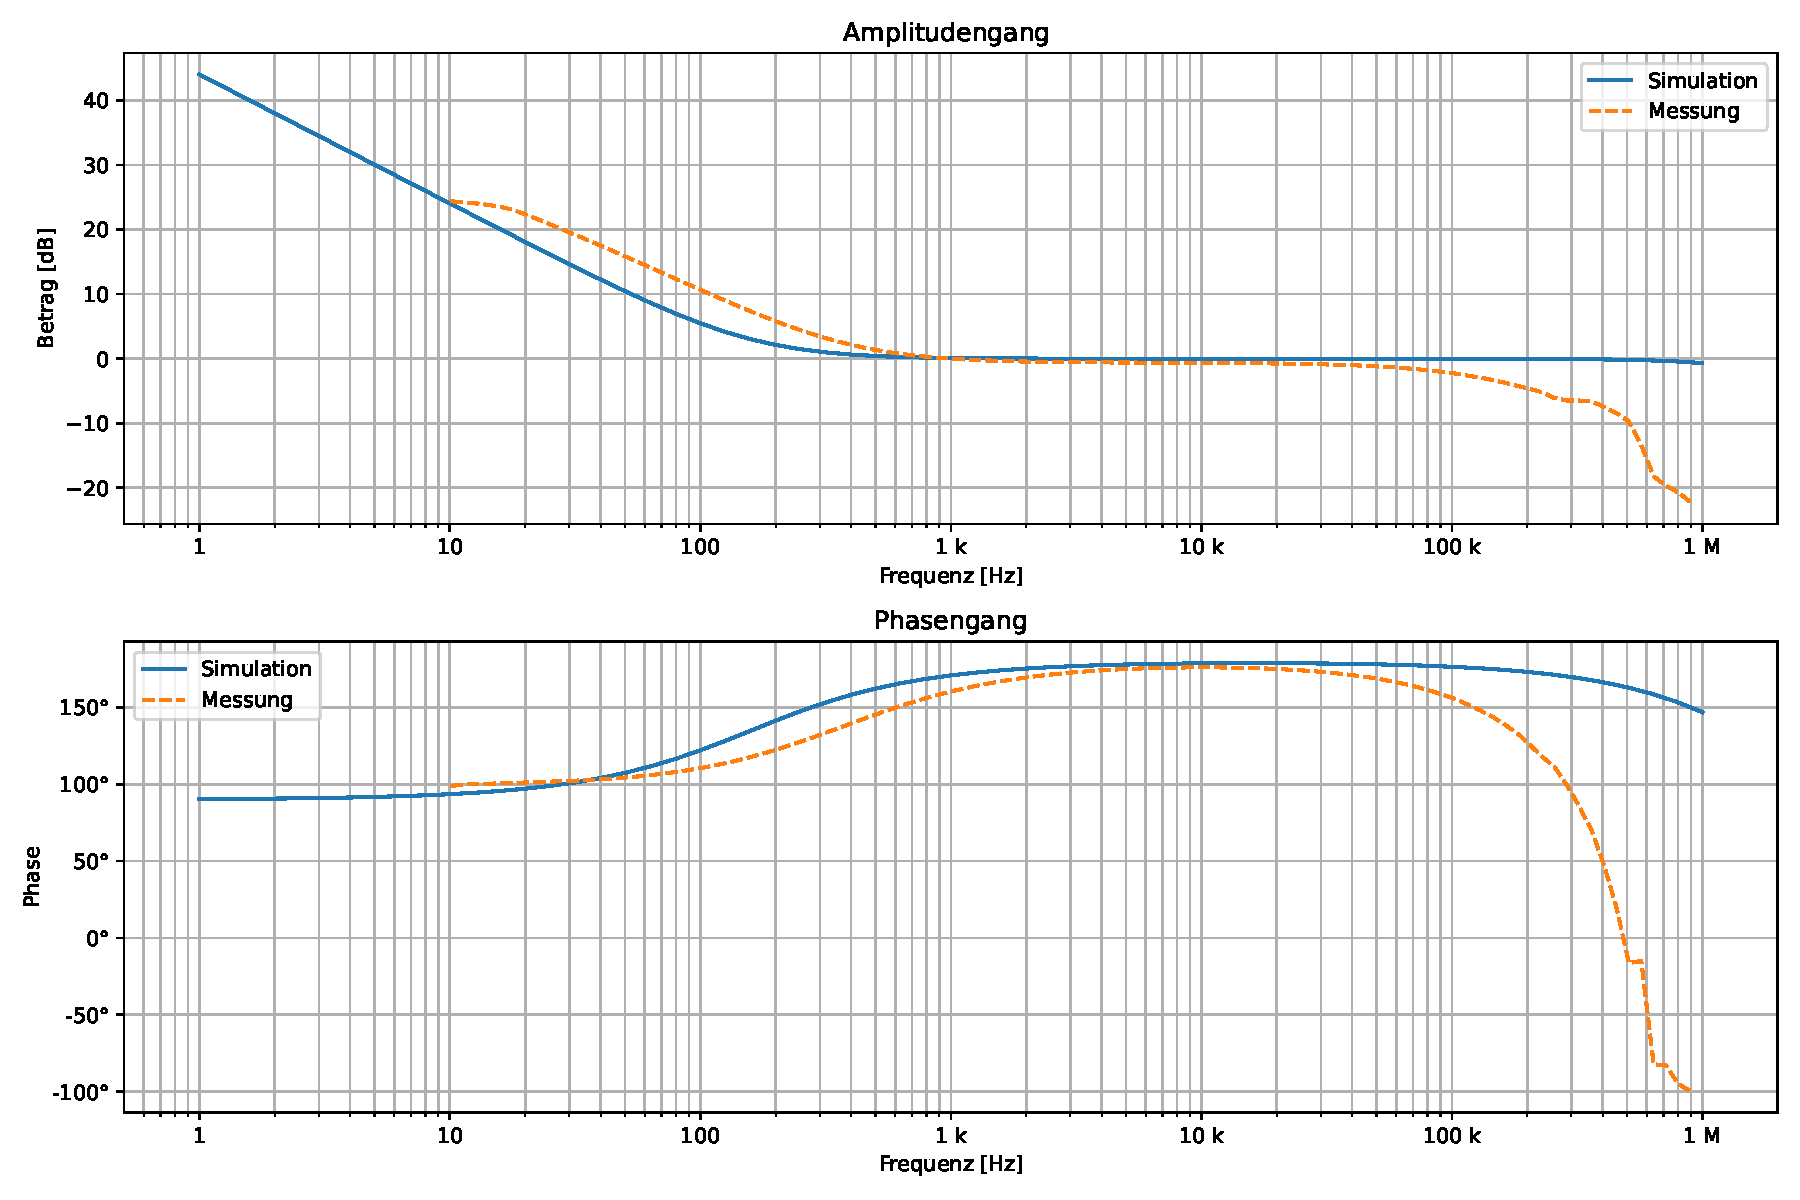
\includegraphics[width=0.8\linewidth]{Elektronik-Laborprotokoll_Filter/Plots/PI_Filter_Bodediagramm_Simulation_mit_Messung.pdf}
  \caption{PI Filter Bodediagramm}
  \label{fig:PI_Filter_Bodediagramm}
\end{figure}
%
Das Bodediagramm des gemessenen PI-Filters weist ein sehr ähnlicher Verlauf wie des simulierten PI\_Filters.

Die Übertragungsfunktion eines PI Filters hat die folgende Form \cite{Skript}:
\begin{equation}
  H_{PI}(s) = \frac{sR_2C + 1}{sR_1C}
\end{equation}




Bei dem PI Filter ist die Amplitudenverstärkung für tiefere Frequenzen größer. Wenn sich die Frequenz des Eingangssignals an die \SI{0}{\hertz} nähert, läuft die Verstärkeung des PI-Filters wegen des I-Anteils gegen unendlich. Die Verstärkung des Integrators verringert sich um mit höheren Frequenze. Wenn sich Wenn sich die Frequenz des Eingangssignals an die $\infty$ nähert, läuft die Verstärkeung des PI-Filters gegen \SI{0}{\decibel}, bzw. 1.\\
Die Messwerte stimmmen für Frequenzen bis \SI{100}{\kilo\hertz} gut mit der Simulation überein. Die deutliche Abweichung, was nicht mit der externen Schaltung erklärt werden kann, bei höheren Frequenzen als \SI{100}{\kilo\hertz} ist in die Charakteristik des verwendeten OPVs zurückzuführen.\\

Die Änderung des $R_1$ wird die Amplitudenverstärkung hat einen Einfluss auf die Amplitudenverstärkung. Wenn $R_1$ größer wird, dann ist für gleiche geringe Frequenz eine höhere Amplitudenverstärkung zu beobachten.\\

Die Änderung des $R_1$ wird die Amplitudenverstärkung hat einen Einfluss auf die Amplitudenverstärkung. Mit steigender Größe von $R_2$ wird an eine Verstärkung von \SI{0}{\decibel} schneller erreicht.\\

Wenn $C$ grßer wird, dann erreicht die Phase früher \SI{180}{\degree}. Die Änderung des $C$ hat den selbenn Einfluss auf die Amplitudenverstärkung wie $R_2$. Mit steigender Größe von $C$ wird an eine Verstärkung von \SI{0}{\decibel} schneller erreicht.


In der Abbildung \ref{fig:Sprungantwort simuliert} wurde die simulierte Sprungantwort auch mit ihrer normierten Form dargestellt.


%Sprunganwort Simulation
\begin{figure}[H]
  \begin{subfigure}{0.5\textwidth} % Hier die Breite auf 0.5\textwidth ändern
    \centering
    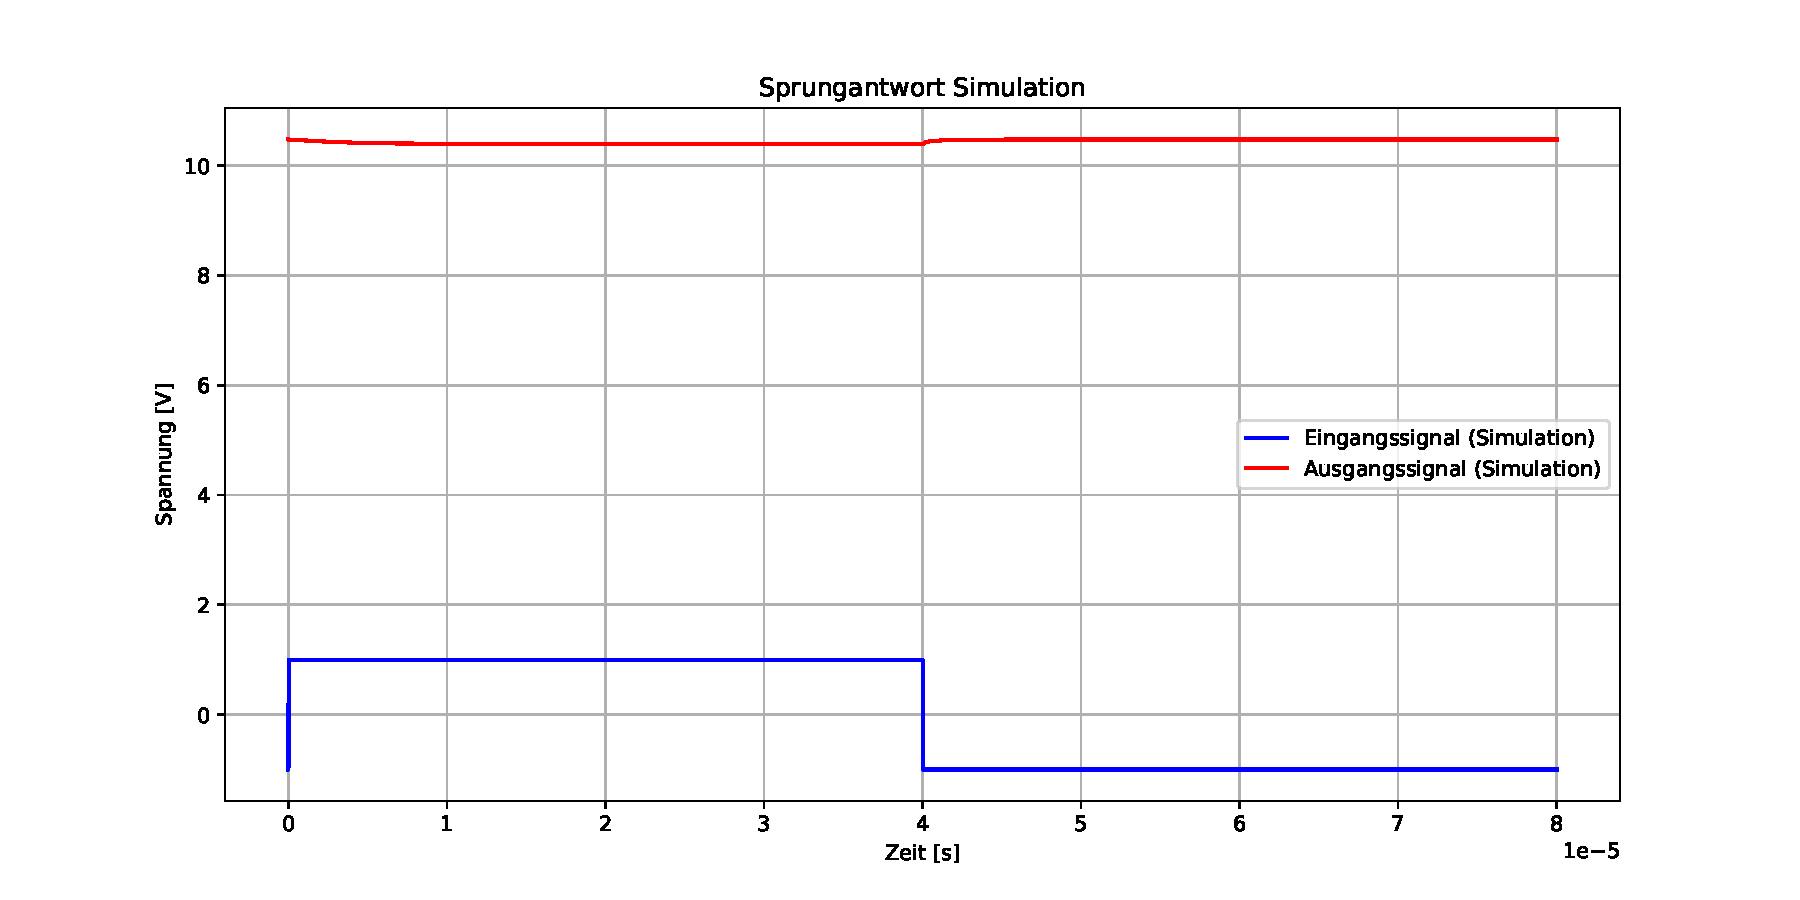
\includegraphics[width=\linewidth]{Elektronik-Laborprotokoll_Filter/Plots/Sprungantwort_Simulation_Plot.pdf}
    \caption{Sprungantwort simuliert}
  \end{subfigure}
  \begin{subfigure}{0.5\textwidth} % Hier die Breite auf 0.5\textwidth ändern
    \centering
    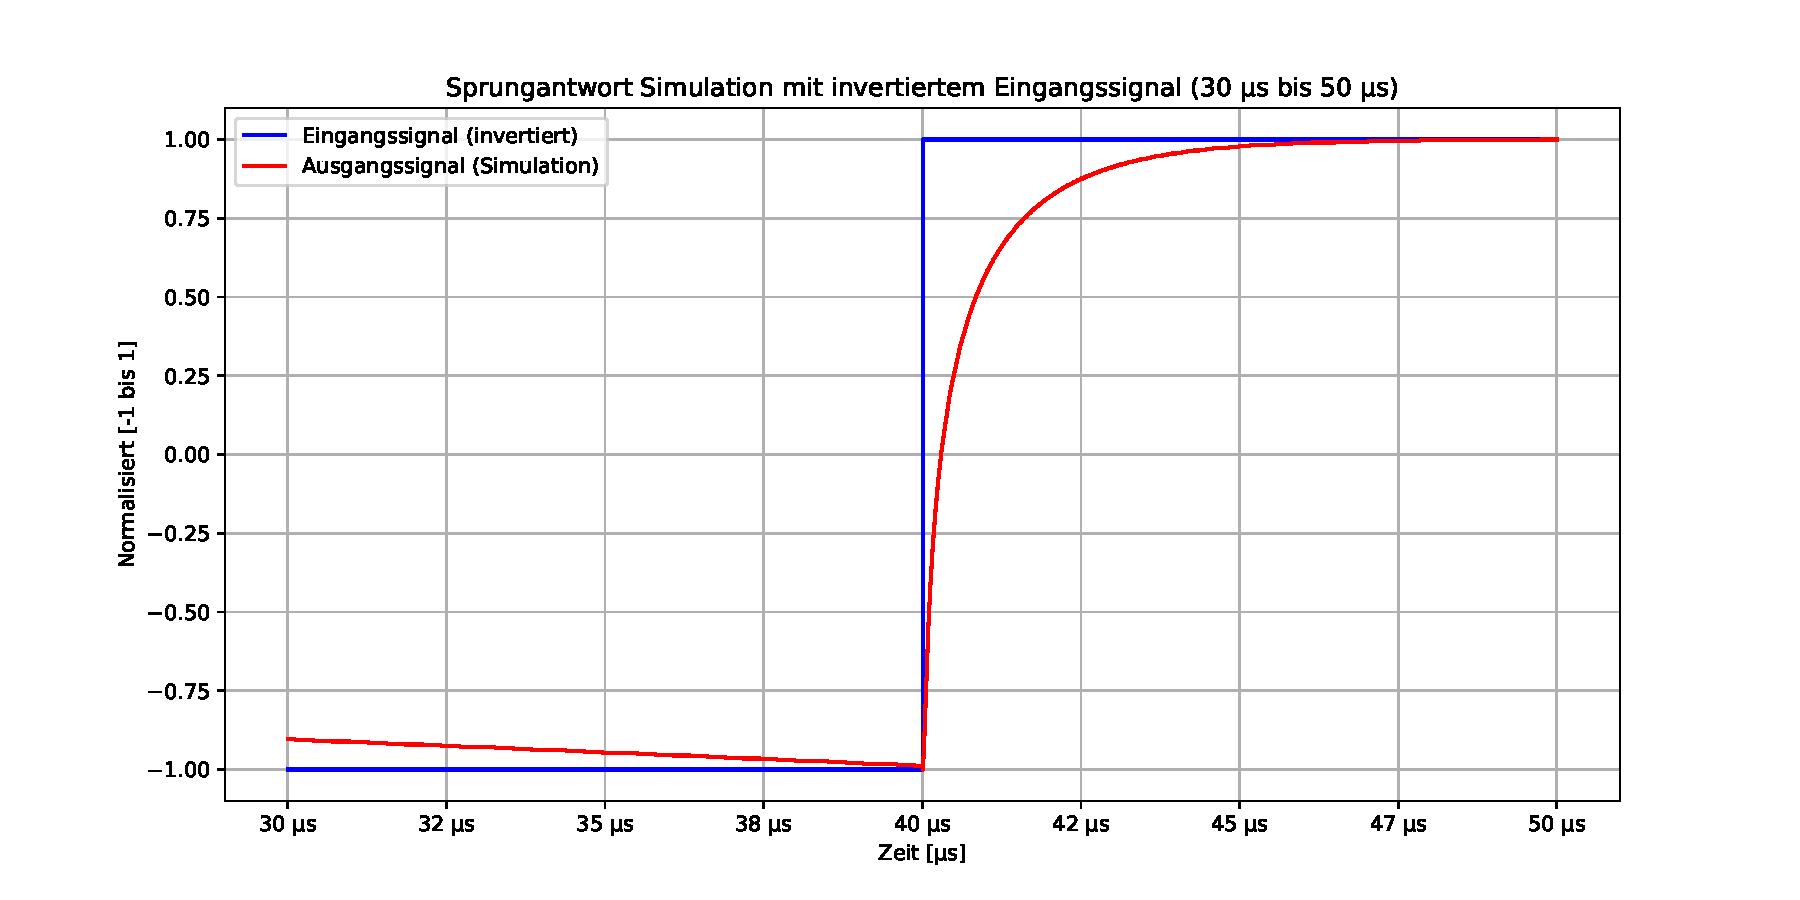
\includegraphics[width=\linewidth]{Elektronik-Laborprotokoll_Filter/Plots/Sprungantwort_Simulation_normiert.pdf}
    \caption{Sprungantwort simuliert normiert}
  \end{subfigure}
 \caption{Sprungantwort (Simulation) }
 \label{fig:Sprungantwort simuliert}
\end{figure}

In der Abbildung der simulierten Sprungantwort zu sehen ist, dass es keine Überschwingen gibt. Die Einstiegszeit dauert ungefähr \SI{2,5}{\micro\second}.\\

In der Abbildung \ref{fig:Sprungantwort gemessen} wurde erstens das Oszilloskopbild dargestellt und dann wurde die Ausgangsspannung invertiert und normiert.

\begin{figure}[H]
  \begin{subfigure}{0.5\textwidth} % Hier die Breite auf 0.5\textwidth ändern
    \centering
    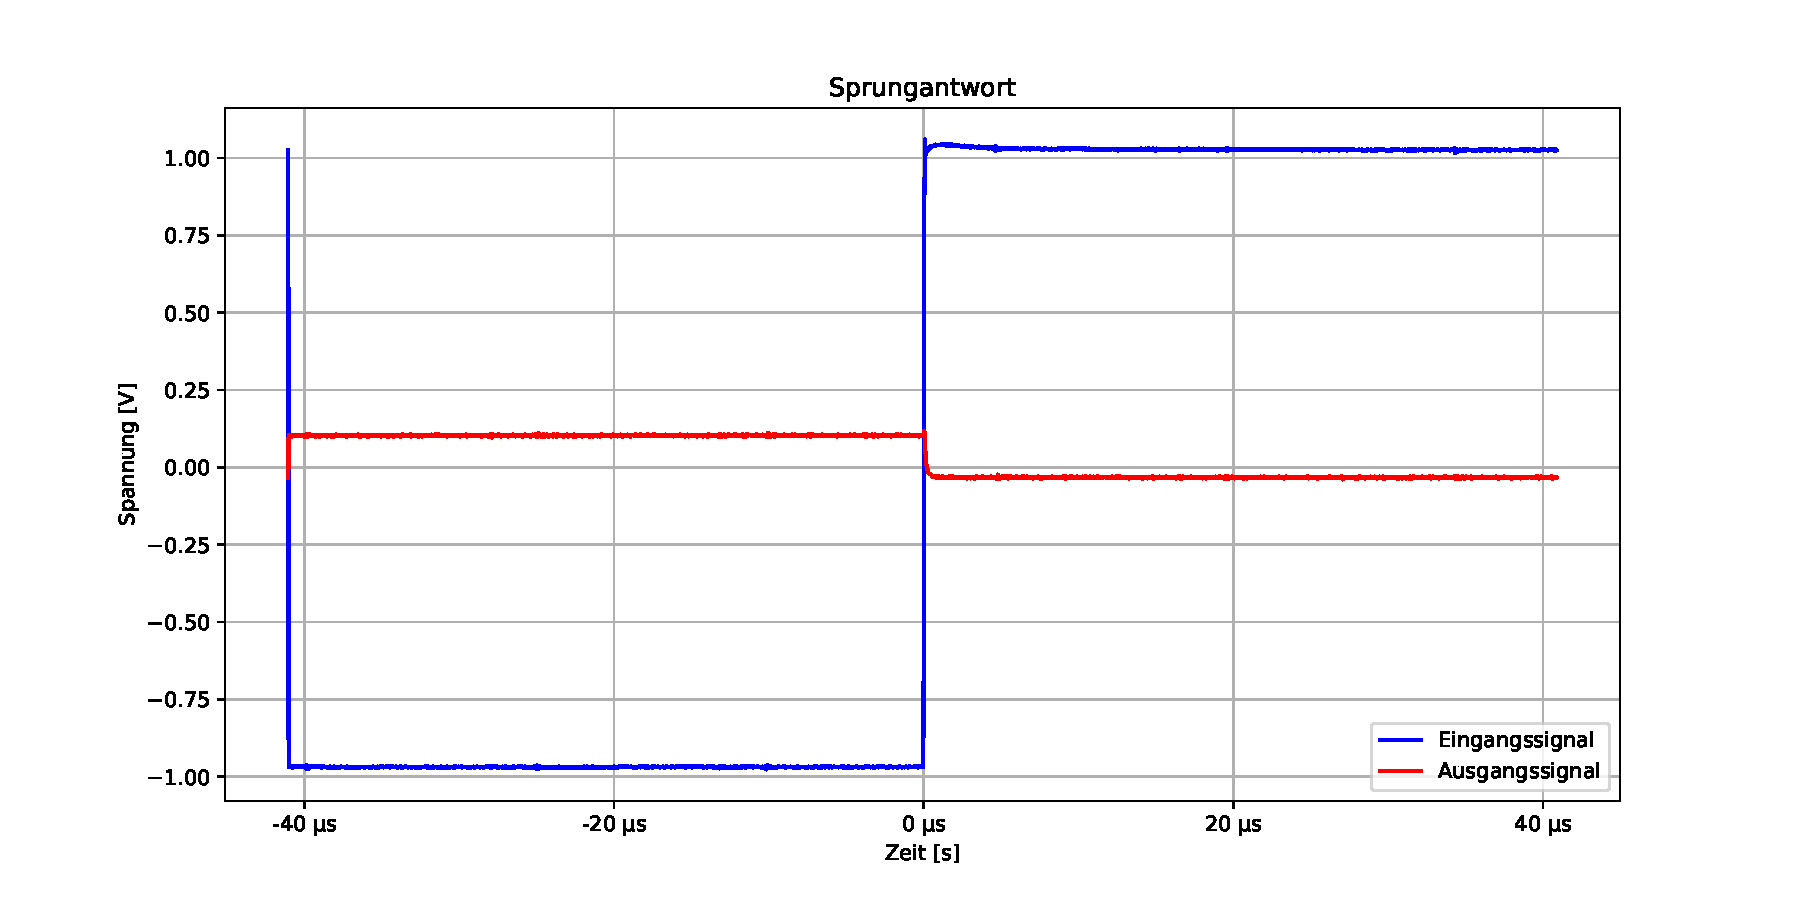
\includegraphics[width=\linewidth]{Elektronik-Laborprotokoll_Filter/Plots/Sprungantwort gemessen.pdf}
    \caption{Sprungantwort gemessen}
  \end{subfigure}
  \begin{subfigure}{0.5\textwidth} % Hier die Breite auf 0.5\textwidth ändern
    \centering
    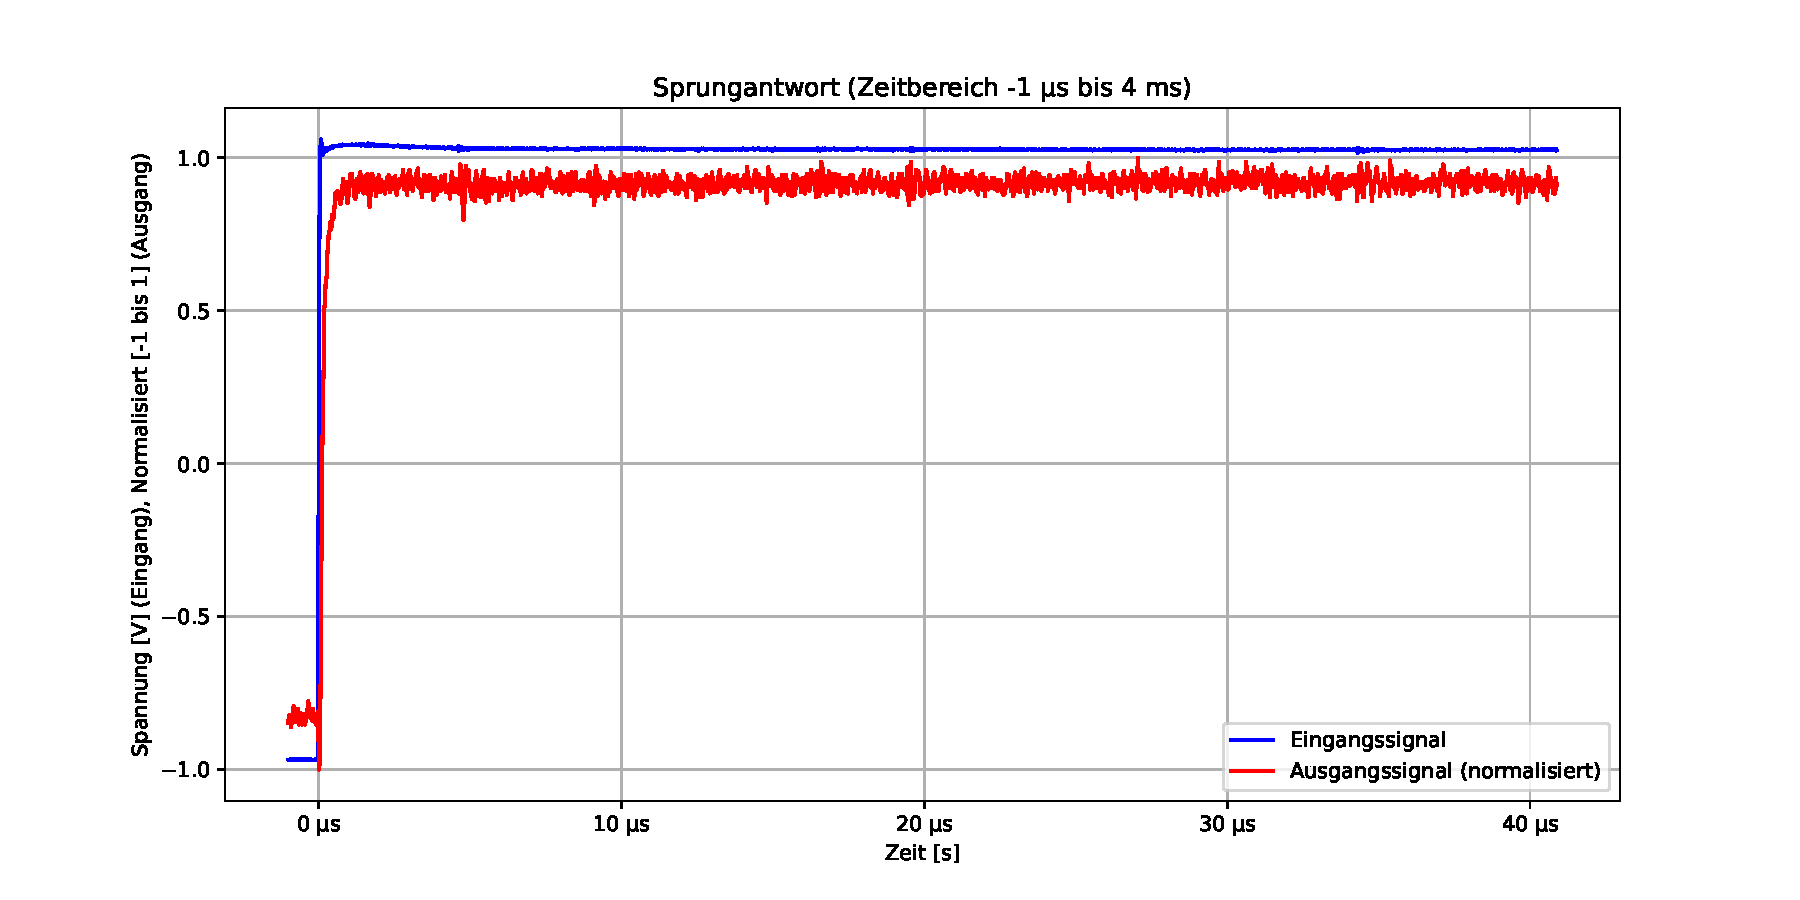
\includegraphics[width=\linewidth]{Elektronik-Laborprotokoll_Filter/Plots/Sprungantwort_gemessen_normiert.pdf}
    \caption{Sprungantowort gemessen normiert}
  \end{subfigure}
 \caption{Sprungantwort (Messung) }
 \label{fig:Sprungantwort gemessen}
\end{figure}

In der Abbildung der gemessenen Sprungantowrt ist  ein Rauschen bei dem Ausgangssignal zu sehen. Trotzdem stimmt die aufgenommene Sprungantwort mit der simulierten gut überein.



%
\subsection{Sallen-Key und MFB}
In der Abbildung \ref{fig:SallenKey_Bode} wurde das Bodediagramm des Sallen-Key-Filters (\ref{fig:Sallenkey_circuit}) für die Simulation-, und Messwerte dargestellt.

\begin{figure}[H]
 \centering
 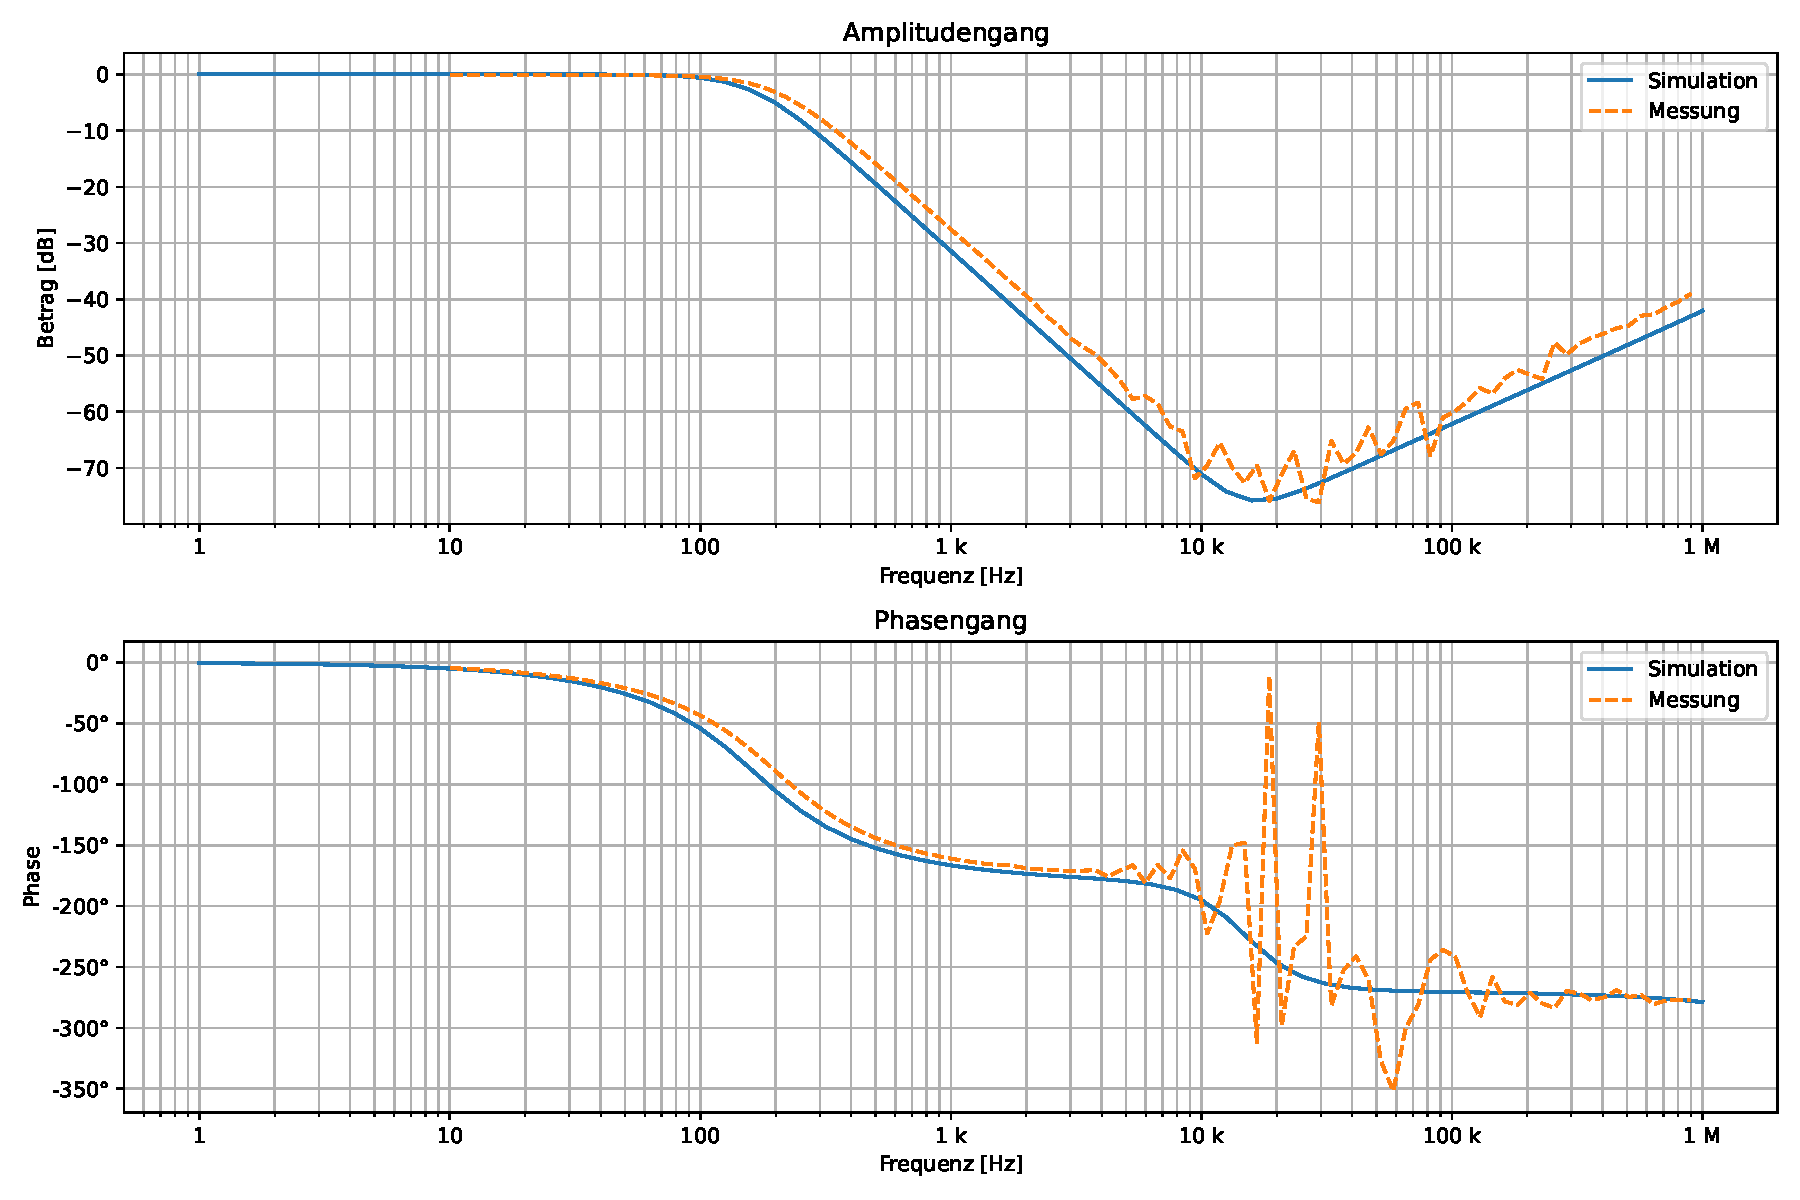
\includegraphics[width=0.7\linewidth]{Elektronik-Laborprotokoll_Filter/Plots/SallenKey_Bodediagramm_Simulation_mit_Messung.pdf}
 \caption{ Bodeplot Sallen-Key-Filter Simulation und  Messung}
 \label{fig:SallenKey_Bode}
\end{figure}

Die Übertragungsfunktion eines Sallen-Key-Filtes hat die folgende Form \cite{Skript}:

\begin{equation}
  H_{SK}(s) = K\frac{ Z_3Z_4}{Z_1Z_2 + Z_4(Z_1 + Z_2 + Z_3) + Z_1Z_3(1 - K)}
\end{equation}

Da es sich um ein Filter 2.Ordnung geht, sollte nach der Theorie die Signale mit geringer Frequenzen als Grenzfrequenz $f_g$ unverändert durch das Filter durchgehen und die höheren Frequenzen. Ab der Grenzfrequenz soll sich die Amplitudenverstärken um \SI{40}{\decibel} pro Dekade verringern.

Aus der Übertragungsfunktion folgt die Formel für die Grenzfrequenz:
\begin{equation}
f_g = \frac{1}{2\pi \sqrt{R_1R_2C_1C_2}}
\end{equation}

Durch die Ersetzung der Werte folgt:

\begin{equation}
f_g = \frac{1}{2\pi \sqrt{\SI{5,6}{\kilo\ohm}\cdot \SI{8,2}{\kilo\ohm}\cdot \SI{100}{\nano\farad}\cdot \SI{205}{\nano\farad}}}\approx \SI{164}{\hertz}
\end{equation}

Das Bodediagramm für Simulation und die Messung bestätigt ebenfalls, dass sich die Grenzfrequenz an der Lage, die nach der Theorie berechnet wurde, befindet.\\

Die Messwerte stimmen mit der Simulation für Frequenzen kleiner als \SI{10}{\kilo\hertz} gut überein. Ab eine Frequenz von \SI{10}{\kilo\hertz} lässt sich ein starkes Überschwingen bei dem Bodediagramm nach den Messwerten erkennen. Dieses Überschwingen ist ebenfalls in die Charakteristik des OPVs zurückzuführen.

\subsection{Universalfilter (simulativ)}

In der Abbildung \ref{fig:Universalfilter_Bode} wurde das Bodediagramm des simulierten Universal-Filters (\ref{fig:Universal_circuit}) dargestellt.

\begin{figure}[H]
 \centering
 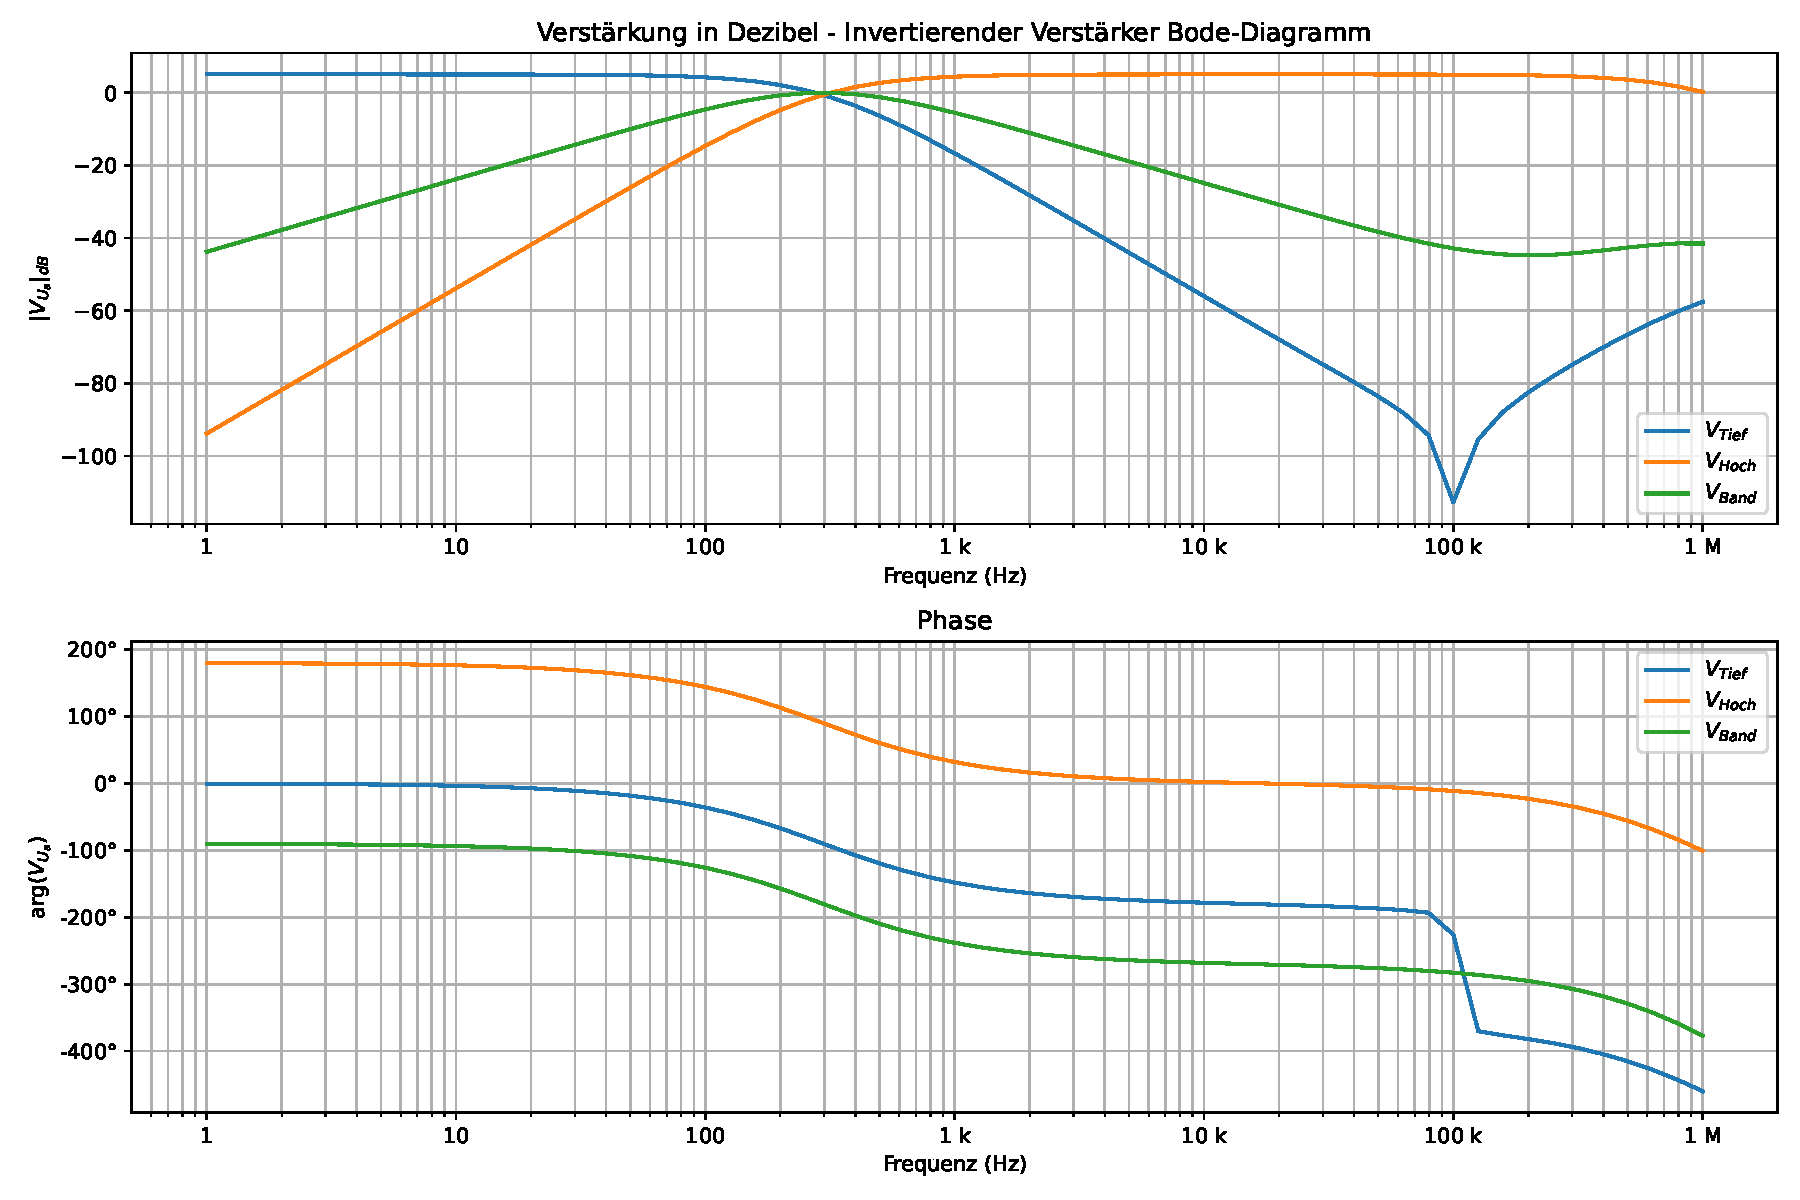
\includegraphics[width=0.7\linewidth]{Elektronik-Laborprotokoll_Filter/Plots/Universalfilter.pdf}
 \caption{ Bodeplot Universal Filter von Simulation }
 \label{fig:Universalfilter_Bode}
\end{figure}

In einem Universalfilter gibt es mehrere Ausgänge (siehe\ref{fig:Universal_Block}) jeweils mit einem Tiefpass-Charakter, einem Hochpass-Charakter und Bandpass-Charakter.Wie in der Abbildung \ref{fig:Universalfilter_Bode} zu sehen ist, haben alle drei Filter ungefähr gleiche Grenzfrequenz $f_g$ .Es ist ebenfalls deutlich erkennbar, dass es einen Unterschied in der Flankensteilheit zwischen Bandpass und anderen beiden Arten gibt. Aus der Phasenantwort lässt sich ablesen, dass sowohl das Hochpass- als auch das Tiefpassfilter invertierend sind, was bedeutet, dass im Durchlassbereich eine Phasenverschiebung von 180° vorliegt.

\begin{figure}[H]
 \centering
 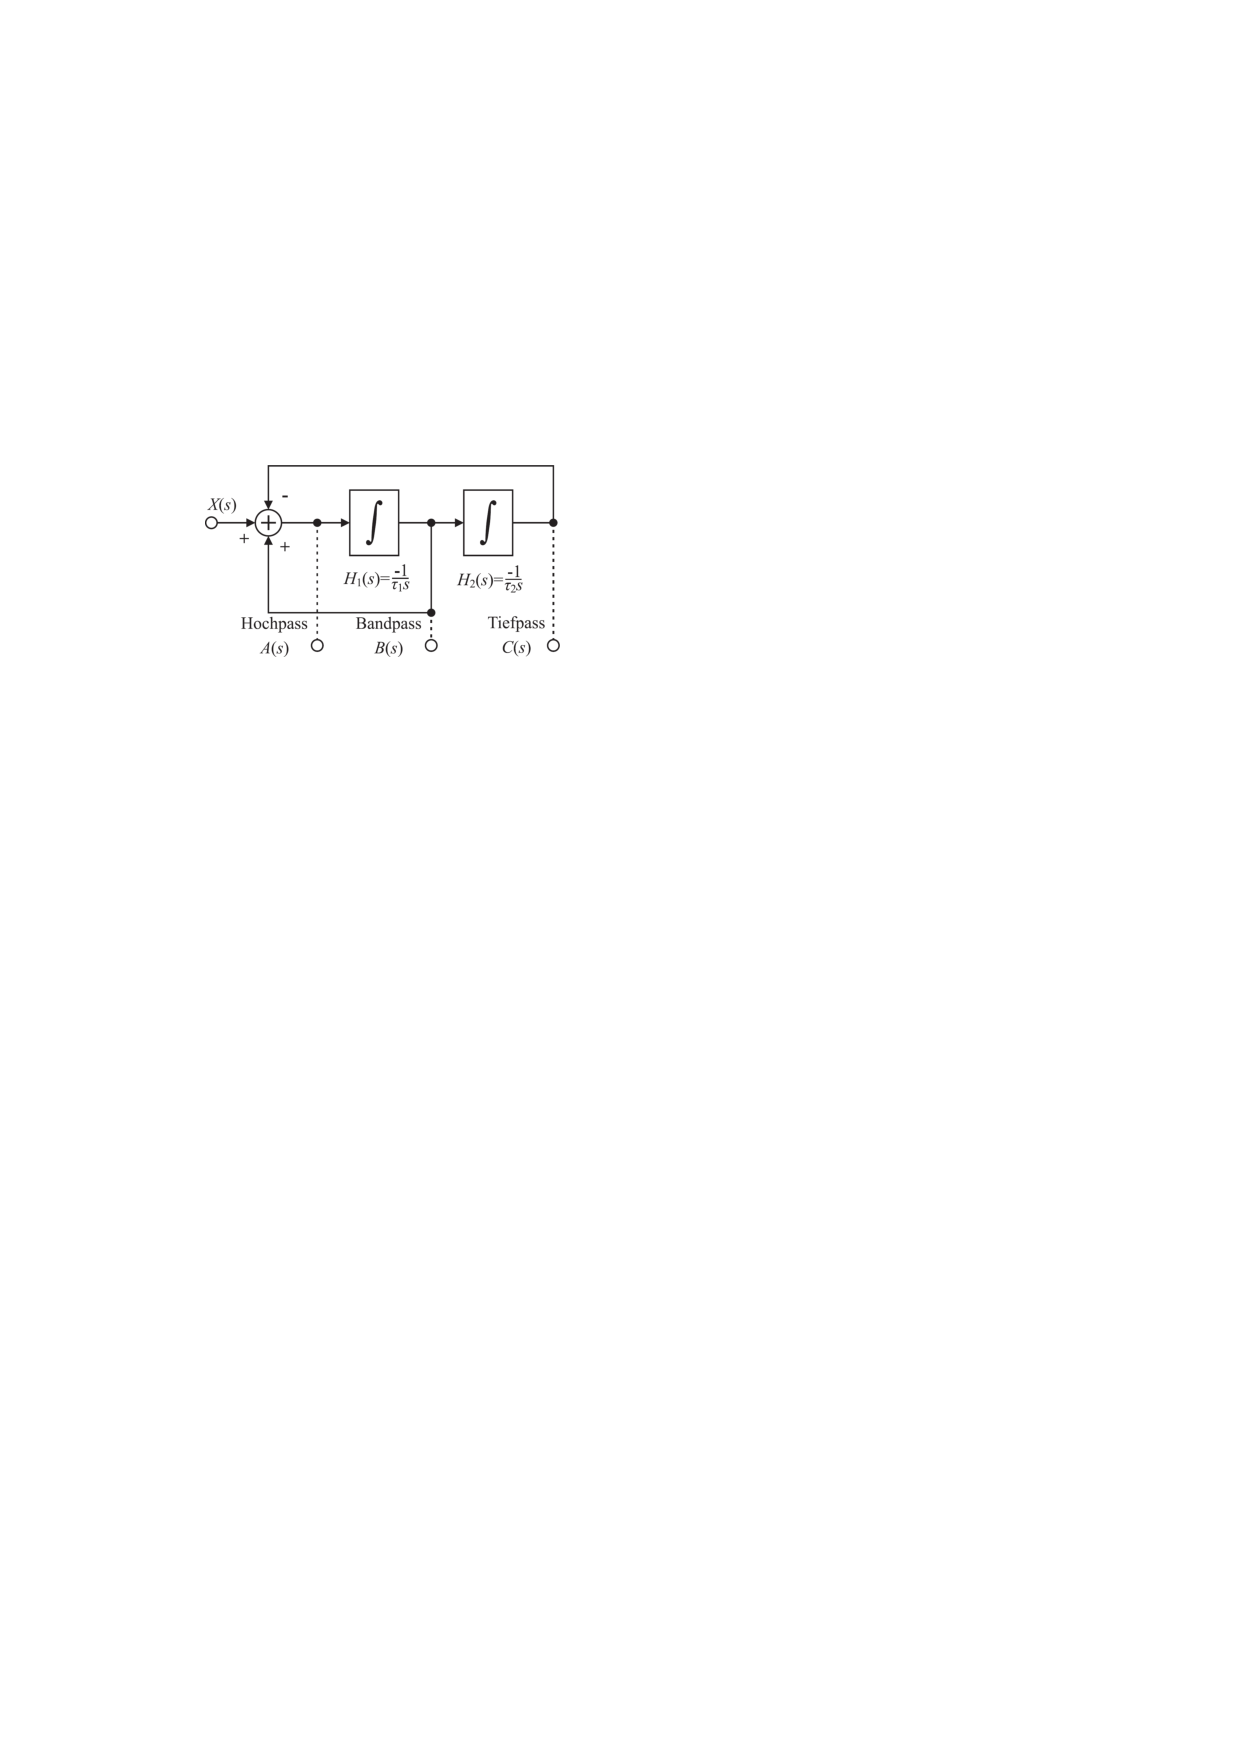
\includegraphics[width=0.7\linewidth]{Elektronik-Laborprotokoll_Filter/Plots/Universalfilter_Block.pdf}
 \caption{ Blockschaltbild für Universalfilter \cite{Skript} }
 \label{fig:Universal_Block}
\end{figure}


\subsection{Allpass und Phasenkompensatoren}

In der Abbildung \ref{fig:Allpass} wurde das Bodediagramm des simulierten Allpass-Filters (\ref{fig:Allpass_circuit})  dargestellt. Im selben Diagramm befindet sich Plots für die Grundschaltung des Allfassfilters und auch die erweiterte Schaltung bzw. der Allpassfilter mit einem Hochpass,der sich im positiven Eingangszweig anstelle des Tiefpassfilters befindet.

%Allpass Diagramm
\begin{figure}[H]
 \centering
 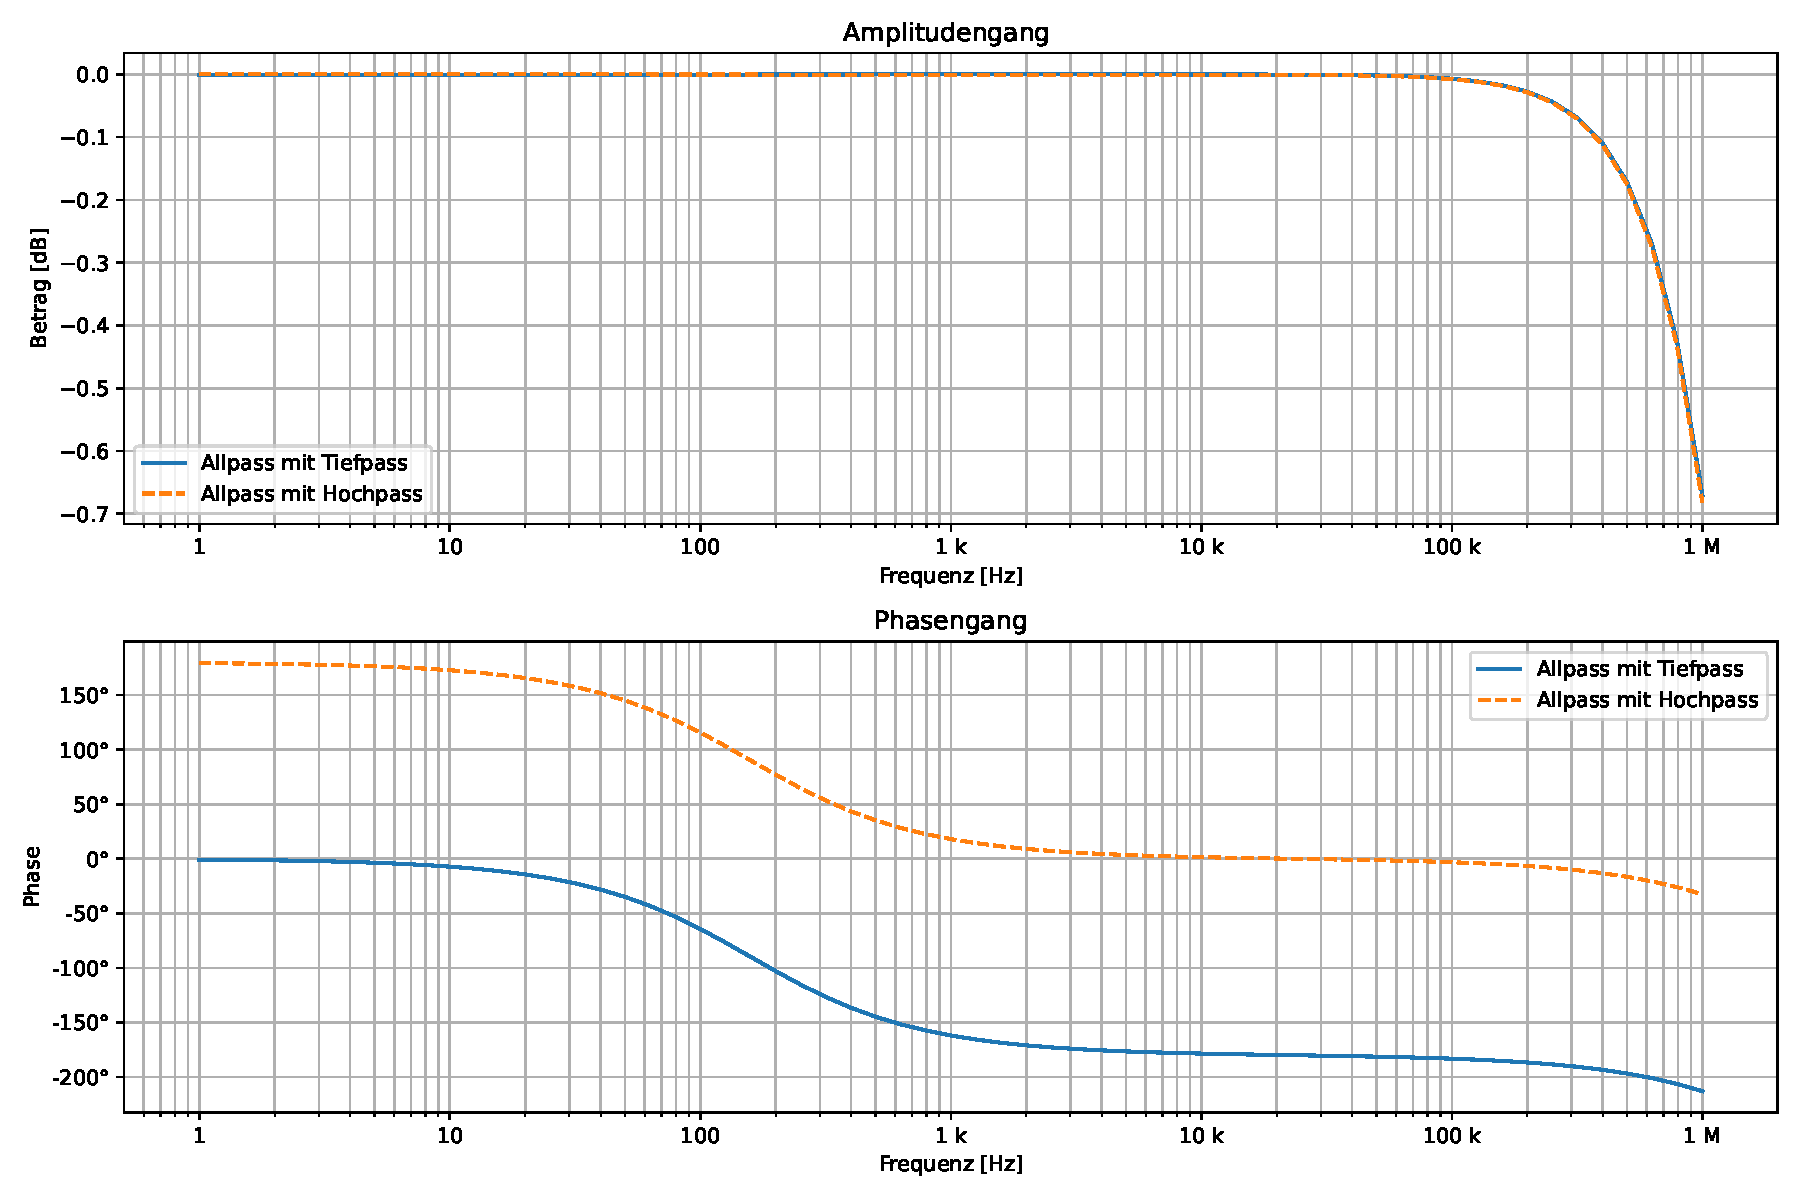
\includegraphics[width=0.7\linewidth]{Elektronik-Laborprotokoll_Filter/Plots/Allpass_Bodediagramm_Simulation_mit_Messung.pdf}
 \caption{Allpass }
 \label{fig:Allpass}
\end{figure}

An dem dargestellten Bodediagramm lässt sich keinen Unterschied bei dem Amplitudengang erkennen, der Einfluss des Hochpassfilter im positiven Eingangszweig ist an dem Phasengang zu bemerken. Die Phase ist im ganzen Diagramm um \SI{180}{\degree} verschoben.\\

In der Abbildung \ref{fig:Phasenkomperator} sind die Graphen für Bessel Tiefpass 3.Ordnung \ref{fig:Bessel_Tiefpass_3.Ordnung} mit und ohne Lag-Kompensator dargestellt.

%Phasenkomperatoren
\begin{figure}[H]
 \centering
 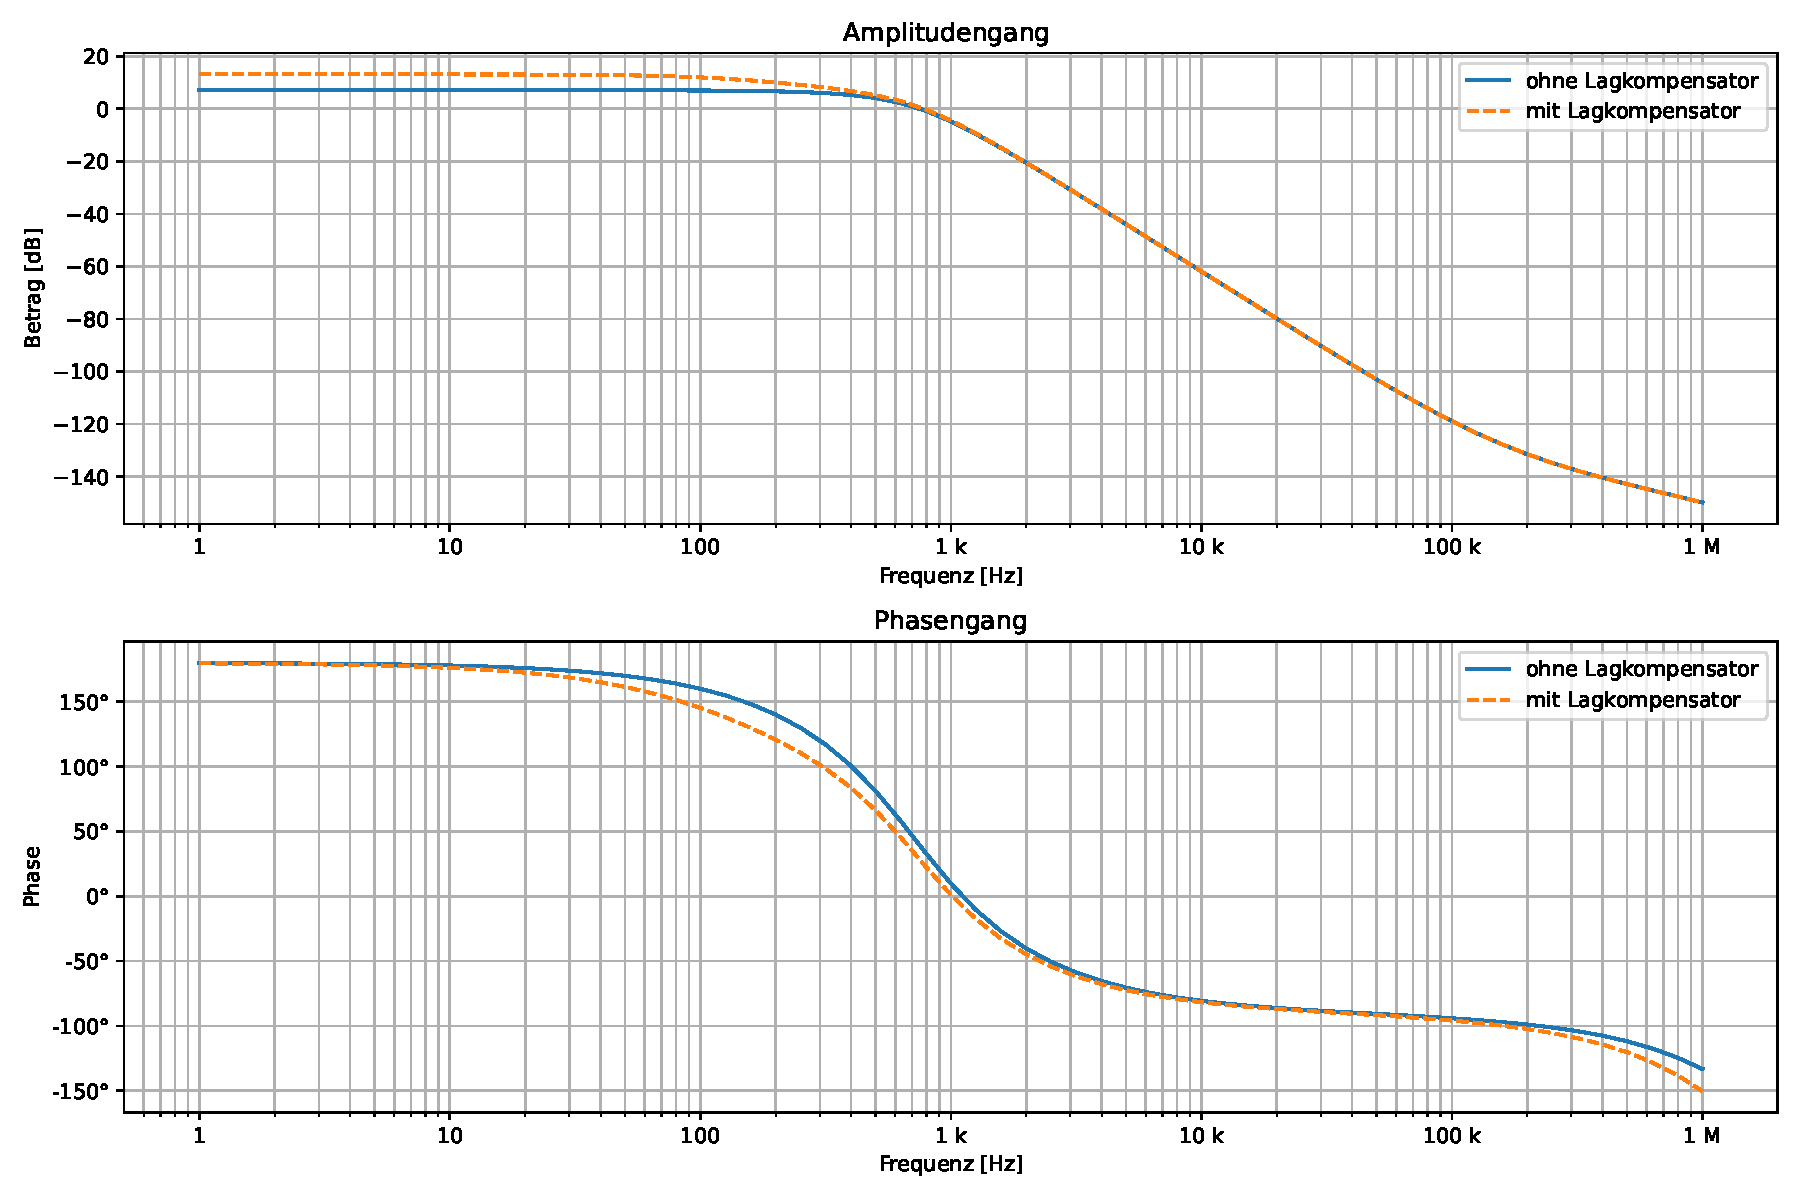
\includegraphics[width=0.7\linewidth]{Elektronik-Laborprotokoll_Filter/Plots/Bode_Phasenkompensatoren.pdf}
 \caption{Phasenkomperator }
 \label{fig:Phasenkomperator}
\end{figure}
%
Der Einfluss des Lag-Kompensators ist für kleinere Frequenzen als \SI{100}{\hertz} zu beobachten. Durch die Verwendung des Lag-Kompensators entsteht sogar eine Amplitudenverstärkung größer als 1 für Frequenzen, die kleiner als $f_g$ sind.\\

Bei dem Phasengang ist der Einfluss des Lag-Komopensators im Bereich zwischen \SI{10}{\hertz} und \SI{1}{\kilo\hertz} zu beobachten. Man merkt, dass sich die Phase unter Verwendung des Lag-Kompensators in diesem Bereich schneller verringert.



